\documentclass{article}
\title{Faster fuzzy text search of a list}
\author{Ben Bullock}
\date{March 2013}
\usepackage[pdftex]{graphicx}
\begin{document}

\maketitle


In fuzzy text searching of a list of words for the closest match by
Levenshtein edit distance.

Performance of 1/10 second for fuzzy text searching over about 120,000
strings of average length twenty bytes each.

First step is to establish a maximum distance $M$, e.g. an edit
distance of ten, $M=10$. This is large enough to accommodate almost
any kind of spelling mistake. Having a maximum distance allows us to
sidestep the highly computationally expensive dynamic programming
algorithm.

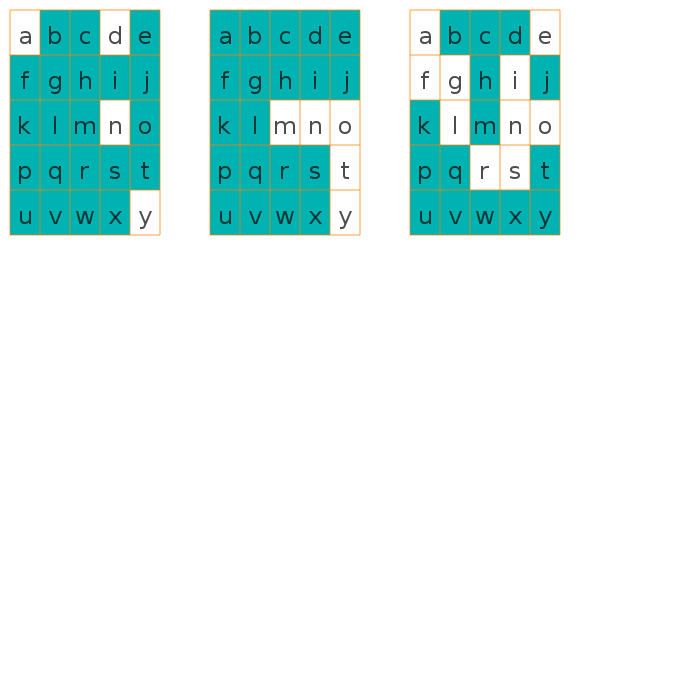
\includegraphics{output.png}

As the list is searched, we keep a track of the lowest distance found
and continually reduce the maximum distance to search for. This means
that a large number of searches can be eliminated.

The first elimination stage is to check the length of the two
strings. If the length of our search term, $L_{S}$, is different
by more than $M$ from the current word being examined, 
$$|L_{S} - L_{w}| > M,$$ 

we know that W cannot be a match for S, and so we can instantly halt
the search.

The next elimination stage relies on generating an alphabet of search
terms for S. If we are searching using bytes, then the alphabet
$\Sigma_S$ needs to be 256 characters in size. Each letter of the
alphabet is marked $1$ if that character is present in S, and $0$ if
that character is not present in S.

Then, W is examined letter by letter to see how many of its letters
are not in the alphabet $\Sigma_S$. If the number of letters in W
which are not in $\Sigma_S$ is greater than $M$, we know that W must
have an edit distance greater than $M$ from S, so we halt the search
and move on to the next term in the list.

If W has the correct length, and its alphabet is sufficiently
coincident with the alphabet of $\Sigma_S$, the next stage is to apply
the dynamic programming algorithm. Since we know the maximum distance
$M$, the dynamic programming algorithm becomes much simpler.

\bf
Extension to Unicode
\rm

\tt Text::Alphabetize \rm

Implementation as \tt Text::Fuzzy\rm.

Application as \tt CPAN::Nearest\rm.

Applications to spell checker, misspelt web page detector.

\bf
References
\rm

\end{document}

